\ifx \globalmark \undefined %% This is default.
	\documentclass[twoside,openright,11pt,a4paper]{report}

%\compiler avec xelatex
%\usepackage[applemac]{inputenc}
\usepackage[T1]{fontenc}
\usepackage[utf8]{inputenc} %latin1 est possible
%\usepackage[latin1]{inputenc} %latin1 est possible
\usepackage[UKenglish]{babel}
\usepackage{lettrine}

%\usepackage[text={13cm,20cm},centering]{geometry}
\usepackage [squaren, Gray, mediumqspace]{SIunits}
\usepackage [top=2cm, bottom=2cm, left=2cm, right=2cm ]{geometry}

\renewcommand{\familydefault}{cmss}
\addto\captionsenglish{ \renewcommand\chaptername{Solutions of Chapte}}

\usepackage{graphicx}
\usepackage{amsmath}
\usepackage{amsfonts}
\usepackage{amssymb}
\usepackage{amsthm}
\usepackage{bm}
\usepackage{color}

\newcommand{\real}{\mathbb{R}}
\newcommand{\mb}{\mathbf}
\newcommand{\bos}{\boldsymbol}

\def \RR {I \! \! R}

\newcommand{\e}{\begin{equation}}  
\newcommand{\ee}{\end{equation}}
\newcommand{\eqn}{\begin{eqnarray}} 
\newcommand{\eeqn}{\end{eqnarray}} 
\newcommand{\eqnn}{\begin{eqnarray*}} 
\newcommand{\eeqnn}{\end{eqnarray*}} 

\newcommand{\bpm}{\begin{pmatrix}}
\newcommand{\epm}{\end{pmatrix}}

%\newcommand{\{\c c}}{\c c}

\newcommand{\bma}{\left(\begin{array}}
\newcommand{\ema}{\end{array}\right)} 
\newcommand{\hh}{\hspace{2mm}}
\newcommand{\hd}{\hspace{5mm}}
\newcommand{\hu}{\hspace{1cm}}
\newcommand{\vv}{\vspace{2mm}}
\newcommand{\vd}{\vspace{5mm}}
\newcommand{\vm}{\vspace{-2mm}}
\newcommand{\teq}{\triangleq}
%\newcommand{\qedb}{\,$\Box$}
\newcommand{\blanc}{$\left. \right.$}
\newcommand{\frts}[2]%
         {\frac{{\textstyle #1}}{{\textstyle #2}}}

\newcommand{\bindex}[3]%
{
\renewcommand{\arraystretch}{0.5}
\begin{array}[t]{c}
#1\\
{\scriptstyle #2}\\
{\scriptstyle #3}
\end{array}
\renewcommand{\arraystretch}{1}
}

\theoremstyle{definition}
\newtheorem{exemple}{{\bf Exemple}}[chapter]
\newtheorem{theoreme}[exemple]{{\bf Th{é}or{è}me}}
\newtheorem{propriete}[exemple]{{\bf Propri{é}t{é}}}
\newtheorem{definition}[exemple]{{\bf D{é}finition}}
\newtheorem{remarque}[exemple]{{\bf Remarque}}
\newtheorem{remarques}[exemple]{{\bf Remarques}}
\newtheorem{lemme}[exemple]{{\bf Lemme}}
\newtheorem{hypothese}[exemple]{{\bf Hypoth{è}se}}
\newtheorem{exercice}{{\bf Exercice}}[chapter]

\newcommand{\xqedhere}[2]{%
 \rlap{\hbox to#1{\hfil\llap{\ensuremath{#2}}}}}

\newcommand{\xqed}[1]{%
 \leavevmode\unskip\penalty9999 \hbox{}\nobreak\hfill
 \quad\hbox{\ensuremath{#1}}}

\newcommand{\gf}{\fg\,\,}

\newcommand{\cata}[1] %
     {\renewcommand{\arraystretch}{0.5}
     \begin{array}[t]{c} \longrightarrow \\ {#1} \end{array}
     \renewcommand{\arraystretch}{1}}

\usepackage[isu]{caption}
%\usepackage[font=small,format=plain,labelfont=bf,up,textfont=it,up]{caption}
\setlength{\captionmargin}{60pt}

\newcommand{\cqfd}
{%
\mbox{}%
\nolinebreak%
\hfill%
\rule{2mm}{2mm}%
\medbreak%
\par%
}

\pagestyle{headings}

\renewcommand{\sectionmark}[1]{%
\markright{\thesection.\ #1}{}}

\renewcommand{\chaptermark}[1]{%
\markboth{\chaptername\ \thechapter.\ #1}{}}

\makeatletter 
\def\@seccntformat#1{\csname the#1\endcsname.\;} 
\makeatother

\title{ {\Huge {\textbf{Modélisation et analyse  \\ \vspace{4mm} des systèmes dynamiques }}} \\ \vspace{4cm} G. Bastin}

%\title{ {\Huge {\textbf{Modelisation et analyse  \\ \vspace{4mm} des systemes dynamiques }}} \\ \vspace{4cm} G. Bastin}


\date{\today}
	\begin{document} %% Crashes if put after (one of the many mysteries of LaTeX?).
\else 
	\documentclass{standalone}
	\begin{document}
\fi

\graphicspath{ {Chapitre1/images/} }

\setcounter{chapter}{0}
\chapter{Systèmes dynamiques et modèles d'état}
\chaptermark{Systèmes dynamiques et modèles d'état}


\lettrine[lines=1]{\bf D}{}ans ce premier chapitre nous donnons tout d'abord la définition de la classe des systèmes dynamiques qui est étudiée dans le livre, ainsi que la terminologie et les notations utilisées, et nous l'illustrons avec divers exemples relevant des sciences de l'ingénieur. Nous expliquons ensuite ce que recouvrent les notions de modélisation et d'analyse des systèmes dynamiques. Le chapitre se termine par une description succincte du contenu des neufs autres chapitres qui constituent le livre.

\section{Définition et exemples} \label{exemple}

Dans ce livre, nous étudierons des systèmes 
dynamiques décrits par des ensembles d'équations différentielles du premier
ordre de la forme
\eqn
\dot x_1&=&f_1(x_1,x_2, \ldots, x_n,u_1,u_2, \ldots u_m), \nonumber\\
\dot x_2&=& f_2(x_1,x_2, \ldots, x_n,u_1,u_2, \ldots u_m), \nonumber\\
\vdots&&\vdots\label{eq:modetn}\\
\dot x_n &=& f_n(x_1,x_2, \ldots, x_n,u_1,u_2, \ldots u_m), \nonumber
\eeqn
où les $f_i$ sont des applications de $\real^{n+m}$ dans $\real$ tandis que les $x_i$ et $u_i$ sont des fonctions scalaires du {\em temps} $t$, qui est une variable indépendante. La quantité $\dot x_i$ représente la dérivée de la variable $x_i$ par rapport au
temps $t$.  Les variables $x_1, x_2, \ldots, x_n$ sont appelées {\em variables
d'état} et contiennent toute l'information nécessaire sur {\em l'état} du
système à l'instant présent pour pouvoir calculer l'évolution de
celui-ci dans le futur, au moyen des équations (\ref{eq:modetn}), étant
données les valeurs futures des variables $u_1, u_2, \ldots, u_m$. 
Celles-ci, appelées {\em entrées} du système, représentent l'influence de l'environnement extérieur sur le système étudié.  On écrit souvent, de manière condensée,  
\e
\dot x = f(x,u)\label{eq:modet}
\ee
où $f$ est une application de $\real^{n+m}$ dans $\real^n$ tandis que $x$ et $u$ sont des fonctions vectorielles du temps. 

Un tel système
d'équations est appelé {\em modèle d'état}. L'objet de ce livre est de traiter
la {\em modélisation}, c'est à dire l'obtention de telles équations dans diverses applications des sciences de l'ingénieur, et {\em l'analyse}, c'est à dire la détermination
des propriétés principales de ces systèmes, déduites des équations.  Nous
commençons par quelques exemples pour illustrer notre propos.
\vv

\begin{exemple}{\bf  Un four de verrerie}

Le premier exemple est un procédé industriel, illustré schématique\-ment
à la figure \ref{fig:fourverre}.  
\begin{figure}[t]
\begin{center}
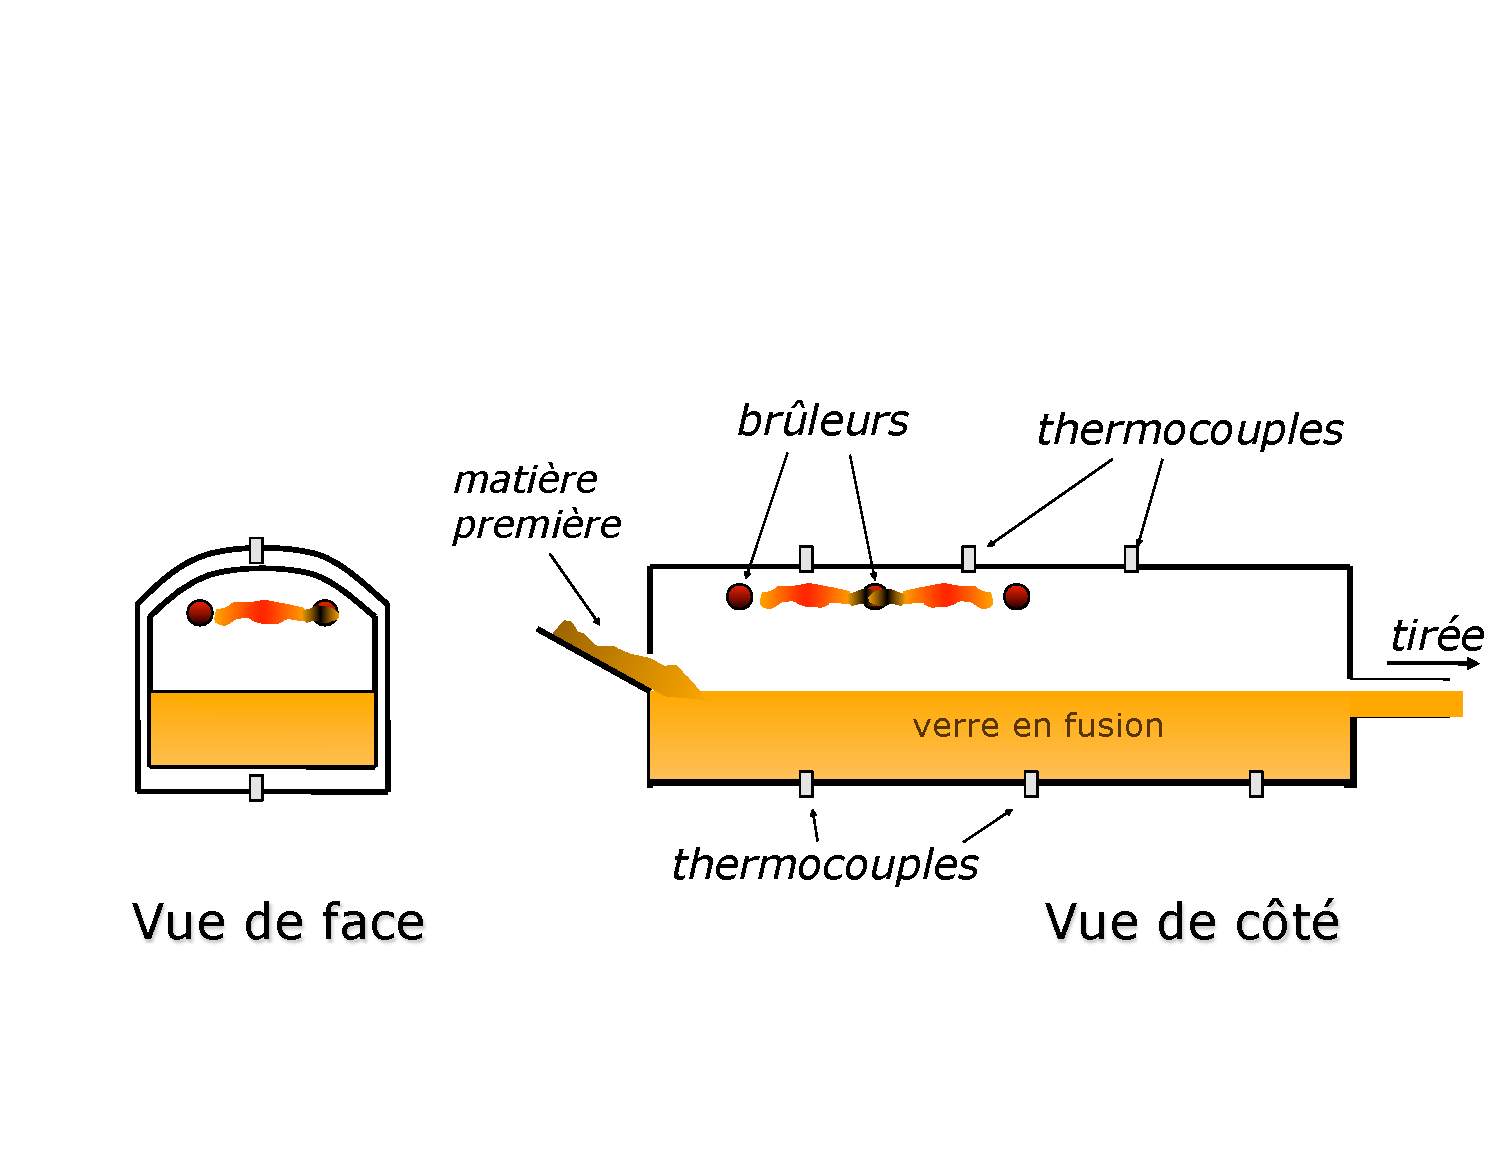
\includegraphics[width=12cm]{fouraverre}
\caption{Four de verrerie}
\label{fig:fourverre}
\end{center}
\end{figure}
Il s'agit d'un four dont les parois sont construites en matériau réfractaire et dans lequel on fait fondre un mélange
de sable, de chaux et d'autres additifs pour obtenir du verre.  Cette fusion est
obtenue par un apport énergétique à l'intérieur du four, provenant par
exemple de brûleurs à gaz disposés au dessus du bain de
verre.  Le verre fondu est extrait du four de manière continue
pour alimenter les machines en aval.  En faisant l'hypothèse que la température du verre est homogène dans
le four et que celui-ci est parfaitement isolé, nous pouvons écrire les deux
équations suivantes, correspondant à un bilan massique et à un bilan énergétique du
procédé. Nous écrivons donc que la variation de masse ou d'énergie, par unité de temps, dans le système considéré est égale à la
somme de  ce qui rentre dans le système, en termes de masse et de chaleur,
diminuée ce qui en sort, toujours durant la même unité de temps:  
\eqn \begin{split}
\frac{dM}{dt} &= P_{in} - P_{out}, \label{eq:bvf} \\
\frac{d}{dt}(CTM) &= Q_{in} + C_{in}T_{in}P_{in}-CTP_{out},
\end{split} \eeqn
avec la signification suivante des variables et paramètres du modèle:\\

$M$ : masse du verre en fusion dans le four (kg),

$T$ : température du verre en fusion dans le four (K),

$T_{in}$ : température de la matière première enfournée (K),

$C$ : chaleur spécifique du verre (J/K$\times$kg),

$C_{in}$: chaleur spécifique de la matière première (J/K$\times$kg),

$Q_{in}$ : quantité de chaleur fournie par unité de temps (J/s),

$P_{in}$ : masse enfournée par unité de temps (kg/s),

$P_{out}$ : masse \og tirée \fg~par unité de temps (kg/s).\\

\noindent Nous avons indiqué des unités pour chacune des grandeurs définies ci-dessus. La cohérence dimensionnelle des équations est la première vérification à effectuer dans un exercice de mise en équation d'un modèle mathématique.

Pour mettre le système d'équations (\ref{eq:bvf}) sous la forme d'un modèle d'état (\ref{eq:modetn}), on définit les variables d'état~:\\

$x_1 \triangleq M$ : masse du verre en fusion (kg),

$x_2 \triangleq C T$ : quantité de chaleur par unité de masse de verre en fusion (J/kg),\\

\noindent et les variables d'entrée~:\\

$u_1 \triangleq P_{in}$ : masse enfournée par unité de temps (kg/s),

$u_2 \triangleq P_{out}$ : masse tirée par unité de temps (kg/s),

$u_3 \triangleq Q_{in}$ : chaleur fournie par unité de temps (J/s).\\

\noindent On obtient alors le modèle d'état~:
\begin{equation} \begin{split} \label{four1}
\dot x_1 &= u_1 - u_2, \\
\dot x_2 &= \dfrac {u_1(\alpha - x_2) + u_3}{x_1},
\end{split} \end{equation}
où le paramètre constant $\alpha = C_{in}T_{in}$ est la quantité de chaleur de la matière enfournée par unité de masse.

On note que d'autres choix des variables d'état et des variables d'entrée sont possibles (voir exercice 1.2). \qed
\end{exemple}  
\vv

\begin{exemple}{\bf  Un réacteur chimique }

\begin{figure}[ht]
\begin{center}
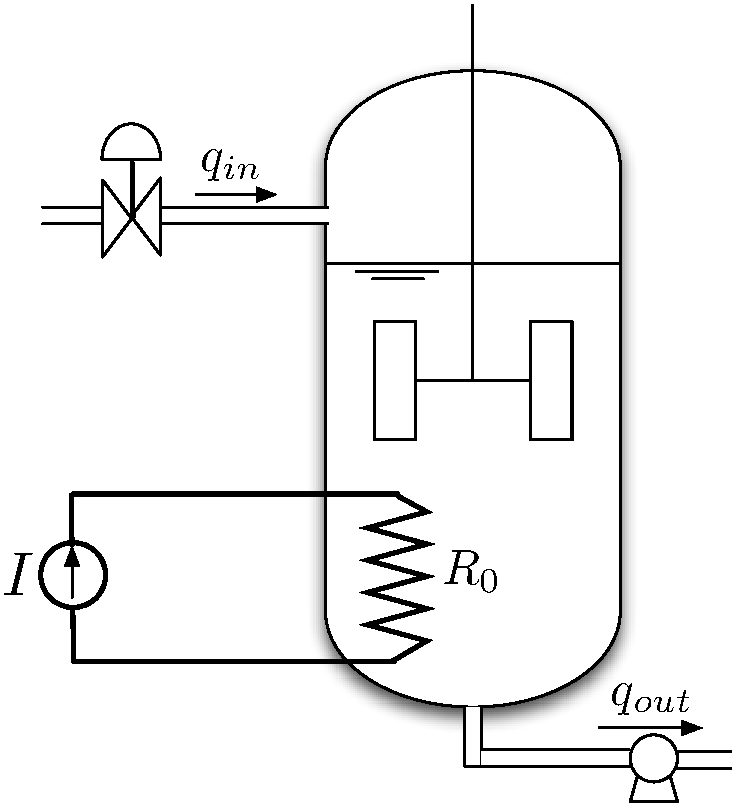
\includegraphics[width=7cm]{reachim}
\caption{Réacteur chimique}
\label{fig:reachim}
\end{center}
\end{figure}
Dans un réacteur chimique (Figure \ref{fig:reachim}), une réaction transformant un réactif A en un produit B se déroule en phase liquide à une certaine température $T$.  Le réacteur est alimenté en réactif
A via une vanne d'alimentation qui introduit le réactif à la concentration
$A_{in}$ avec un débit volumique d'alimentation variable
$q_{in}$ qui est une fonction monotone croissante de l'ouverture de vanne $w$ : $q_{in} = \phi(w)$. Le contenu du réacteur est extrait par une pompe avec un débit de soutirage $q_{out}$. On suppose que la réaction est endothermique et nécessite dès lors un apport calorifique $W$ fourni par une résistance chauffante $R_0$ alimentée par une source de courant variable $I$ comme illustré sur la figure. On suppose en outre que le réacteur est
parfaitement mélangé. La réaction (c.à.d. la transformation du réactif A en
produit B) se passe avec une vitesse de réaction qui obéit à une cinétique du premier ordre, c.à.d. proportionnellement à la quantité de réactif A dans le
réacteur. Le coefficient de proportionnalité est fonction de la température
et vérifie la loi d'Arrhenius, $k(T)=k_0 \exp(-\frac{E}{RT})$.

On décrit l'évolution de ce système en écrivant les équations de bilan volumétrique, massique et thermique:
\begin{equation*} \begin{split} 
&\frac{dV}{dt} = q_{in} - q_{out},\\[0.3em]
&\frac{d}{dt}(AV) = q_{in}A_{in} -q_{out}A-k(T)AV, \\[0.3em]
&\frac{d}{dt}(BV) = -q_{out}B + k(T)AV, \\[0.3em]
&\frac{d}{dt}(CTV) = CT_{in}q_{in}-CTq_{out} - hk(T)AV + R_0I^2,
\end{split} \end{equation*}
avec~:\\

$V$ : volume de liquide dans le réacteur, 

$A$ : concentration en réactif A dans le réacteur,

$B$ : concentration en produit B dans le réacteur,

$k_0$ : constante de vitesse de réaction,

$E$ : énergie d'activation,

$R$ : constante de Boltzmann,

$C$ : chaleur spécifique,

$h$ : enthalpie de réaction.\\

\noindent Les autres notations ont été définies plus haut. En définissant les variables d'état

$x_1 = A$ : concentration en réactif dans le réacteur,

$x_2 = B$ : concentration en produit dans le réacteur,

$x_3 = V$ : volume du milieu réactionnel,

$x_4 = T$ : température du milieu réactionnel,\\

\noindent et les variables d'entrée

$u_1 = w$ : ouverture de vanne,

$u_2 = q_{out}$ : débit de soutirage,

$u_3 = I$ : courant électrique fourni à la résistance chauffante,\\

\noindent on obtient le modèle d'état suivant~:
\begin{equation*} \begin{split} 
\dot x_1 &= \phi(u_1)\dfrac{{\textstyle A_{in} - x_1}}{{\textstyle x_3}} - k(x_4)x_1,\\[0.3em]
\dot x_2 &= - \phi(u_1) \dfrac{x_2}{x_3} + k(x_4)x_1,\\[0.3em]
\dot x_3 &= \phi(u_1) - u_2, \\[0.3em]
\dot x_4 &= \dfrac{{1}}{{x_3}}[\phi(u_1)(T_{in} - x_4) + \dfrac{{R_0}}{{C}}u_3^2] - \dfrac{{h}}{{C}}k(x_4)x_1.
\end{split} \end{equation*}
Les réacteurs {\it continus} et {\it isothermes} constituent un cas particulier intéressant. Il s'agit de réacteurs pour lesquels le volume $V$ et la température $T$ sont maintenus constants par des dispositifs de régulation adéquats. Le modèle d'état est alors réduit aux deux premières équations du modèle ci-dessus~:
\begin{equation} \begin{split} \label{iso}
\dot x_1 &= \dfrac{\phi(u_1)}{{V}} (A_{in} - x_1) - k(T)x_1, \\[0.3em]
\dot x_2 &= - \dfrac{\phi(u_1)}{{V}} x_2 + k(T)x_1.  \xqedhere{4.8cm}{\qed}
\end{split} \end{equation}
\end{exemple}
\vv

\begin{exemple}{\bf Des coccinelles et des pucerons}

Les pucerons sont des insectes ravageurs permanents et redoutables pour les cultures de rosiers. La lutte biologique contre ces ravageurs est une alternative aux traitements par pesticides qui sont de moins en moins efficaces devant les résistances développées par les pucerons. 
\begin{figure}[ht]
\begin{center}
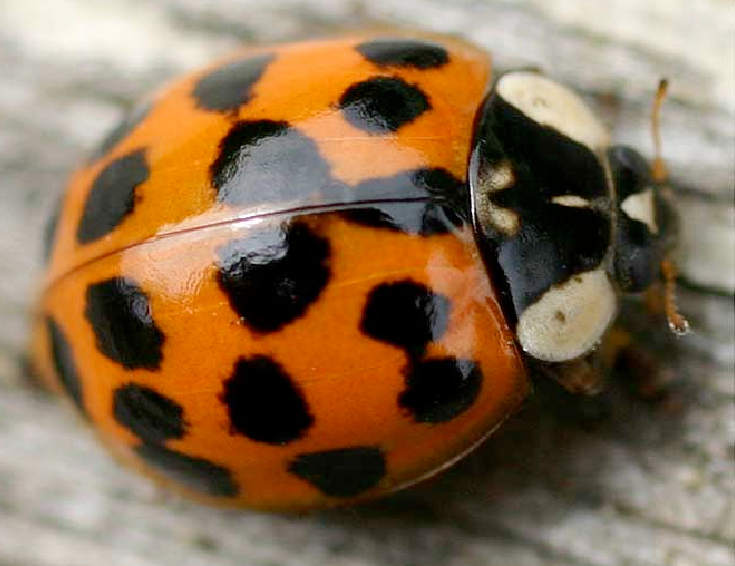
\includegraphics[width=4cm]{cocci}
\caption{Harmonia axyridis}
\label{fig:cocci}
\end{center}
\end{figure}
Les coccinelles {\em Harmonia axyridis} (Fig. \ref{fig:cocci}) sont utilisées dans cette lutte biologique car elles se nourissent de pucerons avec une grande voracité. Elles sont actives dès le printemps, c'est-à-dire dès l'apparition des colonies de pucerons dans les roseraies. Pour augmenter l'efficacité prédatrice des coccinelles, l'Institut Fran\c cais de Recherche Agronomique (INRA) a développé une variété de coccinelles \og sédentaires \gf qui ne volent pas (et ne risquent donc pas de quitter la culture à tra\^ iter).

On souhaite établir un modèle décrivant l'évolution du nombre de pucerons $x_1(t)$ et de coccinelles $x_2(t)$ sous les hypothèses suivantes:
\begin{enumerate}
\item en l'absence de coccinelles, la population de pucerons dispose d'assez de nourriture (les feuilles des rosiers) pour avoir une croissance exponentielle avec un taux spécifique de croissance constant;
\item les coccinelles dévorent d'autant plus de pucerons qu'ils sont nombreux;
\item la prédation par les coccinelles est la seule source de mortalité naturelle des pucerons;
\item les coccinelles ont un taux spécifique constant de mortalité naturelle;
\item le jardinier, qui n'est pas très futé, répand un pesticide qui tue indifférem-ment les pucerons et les coccinelles avec un taux d'épandage variable noté $u(t)$.
\end{enumerate}
Le modèle d'état suivant exprime le bilan du nombre de pucerons et de coccinelles:
\begin{equation} \begin{split}  \label{coc}
\dot x_1 &= ax_1 - bx_1x_2 - cux_1, \\
\dot x_2 &= dx_1x_2 - ex_2 - fux_2. 
\end{split} \end{equation} 
où $a,b,c,d,e,f$ sont des constantes positives. On peut vérifier que chaque terme de ce modèle formalise une des hypothèses ci-dessus. Cette vérification est laissée comme exercice.

Ce type de modèle fut introduit à l'origine par le mathématicien italien V. Volterra qui cherchait à comprendre les fluctuations du rendement de la pêche en mer Adriatique au début du vingtième siècle. Evidemment, il s'agit d'une simplification assez grossière de la réalité. Le modèle ne prend pas en compte de nombreux facteurs qui peuvent influencer l'évolution des populations (conditions climatiques, autres ressources disponibles, autres prédateurs, migration des populations etc ...). Comme l'illustre notre exemple, une application importante de ce type de modèle est la lutte contre les insectes nuisibles dans l'agriculture. Il arrive souvent que la population nuisible soit contr\^olée par l'introduction de prédateurs. Le modèle constitue alors un outil intéressant pour la conception des programmes d'intervention sur le terrain. \qed \\
\end{exemple}


\begin{exemple}{\bf Un moteur à courant continu}

Nous examinons maintenant le dispositif électromécanique illustré à la figure \ref{fig:motdc}.
\begin{figure}[ht]
\begin{center}
\includegraphics[width=6cm]{motdc}
\caption{Moteur à courant continu}
\label{fig:motdc}
\end{center}
\end{figure}
Il s'agit d'un moteur à courant continu qui peut être aussi bien commandé par la tension statorique (ou tension d'excitation) $e$ que par le courant rotorique $I$.
L'équation électrique du circuit statorique est donnée par
\eqnn
e=Ri+L\frac{di}{dt}
\eeqnn
où $R$ et $L$ représentent la résistance et l'inductance du circuit,
$e$ est la tension de commande et $i$ est le courant. Le couple
exercé sur le rotor est donné par $C=\Phi I$ où  $I$ est le courant
rotorique et $\Phi$ est le flux magnétique 
proportionnel au courant d'excitation : $\Phi=Ki$. On obtient donc
\eqnn
C=KiI.
\eeqnn
Il reste à modéliser la partie mécanique de ce système. En notant $\theta$ la
position angulaire du rotor, $J$ son moment d'inertie et  $F$ le coefficient de
frottement visqueux, l'application de la loi de Newton conduit à~:
\eqnn
J\frac{d^2\theta}{dt^2}+F\frac{d\theta}{dt}=C.
\eeqnn

En définissant comme variables d'état $x_1=\theta, x_2=\dot{\theta}, x_3=i$, et
comme entrées $u_1=e$, $u_2=I$, on obtient le modèle d'état suivant:
\begin{equation} \begin{split} \label{motDC}
\dot x_1 &= x_2,  \\[0.3em]
\dot x_2 &= -\frac{F}{J}x_2+\frac{K}{J}x_3u_2, \\[0.3em]
\dot x_3 &= -\frac{R}{L}x_3+\frac{1}{L}u_1. \xqedhere{5cm}{\qed}
\end{split} \end{equation}
\end{exemple}
Les quatre exemples que nous venons de traiter ont pour but de montrer
que l'équation (\ref{eq:modet}) permet effectivement de construire des modèles de systèmes dynamiques dans des domaines variés d'application 
des sciences de l'ingénieur puisque nous avons traité successivement des exemples relevant de la thermodynamique, du génie chimique, de l'écologie et de l'électrotechnique.  Ils permettront aussi de mieux appréhender la terminologie qui est présentée dans la section suivante. 

\section{Terminologie et notations}

Comme les exemples précédents l'ont illustré, nous étudions des {\em systèmes
dynamiques} dont le comportement est décrit par un {\em modèle d'état} formé
d'un ensemble d'équations différentielles écrites sous forme condensée :
\eqn
\dot x = f(x,u). \label{sysdyn}
\eeqn
On considère ce modèle d'état à partir d'un instant initial noté $t_0$. 
L'état $x \in \real^n$ et l'entrée $u \in \real^m$ sont des fonctions vectorielles du
temps que l'on notera parfois $x(t)$ et $u(t)$.  Cependant
l'argument $t$ sera souvent omis sans risque de confusion.

Pour un système donné, l'entrée $u(t)$ est a priori une fonction quelconque du
temps.  On supposera cependant toujours qu'il s'agit d'une fonction {\em continue par morceaux} et {\em
bornée}~: $u(t) \in {\cal U}$ où ${\cal U}$ désigne un ensemble de fonctions continues par morceaux et 
bornées de $\real$ dans $\real^m$.

Pour une valeur donnée de l'état initial $x(t_0) = x_0$ et pour une entrée
$u(t)$ donnée, la solution $x(t) \;\; t \geq t_0$ du système différentiel
(\ref{sysdyn}) est appelée {\em trajectoire} du système.  Parfois, quand ce
sera nécessaire pour la clarté de l'exposé, la trajectoire sera notée
$x(t, x_0, u)$.  Nous supposerons toujours qu'une telle trajectoire existe
à tout instant $t\geq t_0$, est unique et est une fonction continue du temps.
Graphiquement, une trajectoire peut donc être visualisée par une courbe continue dans l'espace $\real^{n+1}$.  La projection de la trajectoire dans
{\em l'espace d'état} $\real^n$ (on dit aussi {\em espace de phase}) est appelée
une {\em orbite} du système.

Lorsque l'entrée $u(t)$ peut être choisie librement dans ${\cal U}$, on dit
que le système $\dot x = f(x,u)$ est un système {\em forcé} ou encore un
système {\em commandé}.  Le qualificatif {\em forcé} est utilisé pour
signifier qu'au départ d'un état initial $x_0$, l'allure de la trajectoire
est en quelque sorte forcée par le choix que l'on a fait d'une entrée $u(t)$. De même, dans un contexte d'automatique, le qualificatif {\em commandé}
signifie que l'état du système peut être piloté dans l'espace d'état par une manipulation appropriée de l'entrée $u(t)$.

Nous serons cependant souvent amenés, dans les chapitres suivants, à nous
intéresser à la solution de l'équation $\dot x = f(x,u)$ lorsque l'entrée est
en réalité une constante fixée a priori : $u(t) = \bar u \;\; \forall t \geq
t_0$.  Dans ce cas, on écrit le modèle d'état sous la forme $\dot x = f(x,
\bar u)$.  Parfois on écrit aussi 
\eqnn
\dot x = f_{\bar u} (x)
\eeqnn
pour exprimer plus clairement que $f$ est une fonction de $x$ seulement,
paramétrée par la constante $\bar u$.  Dans un tel cas, il n'y a évidemment
qu'une seule trajectoire possible évoluant librement au départ d'un état
initial $x_0$.  En fixant d'avance l'entrée à une valeur constante, on se
prive de la possibilité de piloter les trajectoires du système et on dit que
le système est {\em libre} (on dit aussi système {\em autonome} ou système
{\em stationnaire}).  La trajectoire est parfois appelée {réponse libre} du
système.  

Lorsque l'on s'intéresse à la solution de l'équation $\dot x = f(x,u)$ pour
{\em une} entrée $u(t)$ variant au cours du temps mais particulière (par
exemple une sinusoide), on peut tout aussi bien oublier que l'on a
sélectionné cette entrée dans ${\cal U}$ et écrire tout simplement : 
\eqnn
\dot x = f(x,t)
\eeqnn
Un système dynamique représenté de cette manière est appelé système {\em  non
autonome} ou {\em instationnaire}.  

Nous serons parfois amenés à considérer divers cas particuliers du modèle
d'état général (\ref{sysdyn}).  On distinguera notamment~:\\

\noindent \textbf{\textit{Les systèmes affines en l'entrée}}
\eqnn
\dot x = f(x) + \sum^m_{i=1} u_ig_i(x) \triangleq f(x) + G(x)u
\eeqnn
où $f$ et les $g_i$ sont des applications de $\real^n$ dans $\real^n$.
Le modèle d'état \eqref{four1} d'un four de verrerie est de cette forme avec les définitions suivantes~:
\begin{equation*}
f(x) = 0, \hh \hh \hh \hh G(x) = \left(\begin{array}{ccc}
1&-1 & 0 \\[0.3em] (\alpha-x_2)/x_1 & 0 & 1/x_1 \end{array} \right).
\end{equation*}\\

\noindent \textbf{\textit{Les systèmes affines en l'état}}
\eqnn
\dot x = \sum^m_{i=1}x_i a_i(u) + b(u) \triangleq A(u) x + b(u) 
\eeqnn
où $b$ et les $a_i$ sont des applications de $\real^m$ dans $\real^n$. Le modèle d'état d'un réacteur chimique continu isotherme \eqref{iso} est de
cette forme avec les définitions suivantes~:
\begin{equation*} \begin{split}
A(u) &= \left(\begin{array}{cc}
-(\dfrac{\phi(u_1)}{V} +k(T)) & 0 \\[0.3em] k(T) & -\dfrac{ \phi(u_1)}{V}
\end{array} \right),\\[0.5em]
b(u) &=  \left(\begin{array}{c} \dfrac{ \phi(u_1) A_{in}}{V}\\[0.7em] 0
\end{array}\right).
\end{split} \end{equation*}\\

\noindent \textbf{\textit{Les systèmes bilinéaires}}
 
Ce sont des systèmes affines à la fois en l'état et en
l'entrée
\begin{eqnarray*}
\dot x &=& \left ( A_0 + \sum^m_{i=1} u_iA_i \right) x + B_0u, \\[0.3em]
&=& A_0x + (B_0+ \sum^n_{i=1} x_i B_i)u,
\end{eqnarray*}
où les $A_i$ $(i = 0, \ldots, m)$ sont des matrices de dimension $(n
\times n)$ et les $B_i$ $(i = 0, \ldots, n)$ sont des matrices de
dimension $(n \times m)$.  Le modèle d'état d'un moteur à courant continu
(\ref{motDC}) est de cette forme avec les définitions suivantes~:
\begin{equation*} \begin{split}
A_0 &= \left( \begin{array}{ccc}
0 & 1 & 0 \\[0.3em] 0 &-\dfrac{B}{J} & 0\\[0.3em]
0&0& -\dfrac{R}{L}
\end{array}
\right)\;\;\; A_1 = 0
\\
A_2 &= \left( \begin{array}{ccc}
0 & 0 & 0 \\[0.3em] 0 & 0 & \dfrac{K}{J} \\[0.5em]
0 & 0 & 0
\end{array}\right)\hspace*{10mm} B_0 = \left(\begin{array}{cc} 0 & 0 \\[0.3em] 0 & 0 \\[0.3em] \dfrac{1}{L}&0
\end{array} \right).
\end{split} \end{equation*}\\

\noindent \textbf{\textit{Linear systems}}
$$
\dot x = Ax +Bu
$$
where $A$ is a matrix of dimension $(n \times n)$ and $B$ is a matrix of dimension $(n \times m)$.  If we consider the state model of the DC motor assuming that the rotor current source is constant ($I$ = constant), we obtain an example of a linear system with
\begin{equation*}
A = \left( \begin{array}{ccc}
0 & 1 & 0 \\[0.3em] 0 &-\dfrac{B}{J} & \dfrac{KI}{J}\\[0.9em]
0&0& -\dfrac{R}{L}
\end{array}
\right)\;\;\; B = \left(\begin{array}{cc} 0 & 0 \\[0.3em] 0 & 0 \\[0.3em] \dfrac{1}{L}&0
\end{array} \right).
\end{equation*}
\vv

\section{Modeling and analysis}

A dynamic system, as we conceive it in this book, is thus a part of the {\it concrete} reality that seems relevant in an engineering problem and that we choose to isolate in thought to describe its behavior in mathematical terms using a model. In particular, we are interested in characterize quantitatively the evolution over time of the {\it state} of the system. For this, we use \blue{deterministic, lumped parameters state models} which consist of ordinary differential equations.

However, other modeling approaches of dynamic systems are possible. For the various examples described in the section \ref{exemple} we could have  build \blue{deterministic, {\it distributed parameters} state models} composed of partial differential equations. This is how, in the example of the glass furnace, we made the hypothesis that the temperature was uniform across the glass bath. This is a simplistic view, but very useful to build simple and effective models for instance in view of the control and optimization of the dynamic behavior of the furnace. However, if this hypothesis is not accepted and we want to study the spatial variations of temperature, we can develop a state model consisting of partial differential equations describing the evolution over time of the temperature and velocity of the fluid fields in the molten glass bath. Neither model is better than the other. They simply are different models obtained for different objectives, usually corresponding to different spatial and temporal scales.

The interaction between the system and the \og outside world \gf is represented by the inputs of the model $u_i(t)$ which are, as we mentioned above, functions of time, real and deterministic. In reality, a given system is often subject to random influences that can be represented by introducing stochastic inputs, i.e. random functions $u_i(t) $ (also called stochastic processes). We then obtain stochastic state models whose state variables are themselves random functions and whose study uses different mathematical techniques than those used in this book.

The state model of a dynamic system is thus a simplified mathematical representation of the behavior of the system. Yet, when it will not affect the clarity of the argumentation, we will often consider these two notions as equivalent in order to simplify the presentation. We will then speak of the dynamic system $\dot x = f(x,u)$, implying that we actually speak of a deterministic state model of the system.

The {\it modeling} of a dynamic system, as we conceive it in this book, is thus the exercise that aims to, given a discursive and qualitative description of the system, establish a mathematical description of it as a state model. Without being unnecessarily complicated, the resulting model should be an effective tool for solving the engineering problem posed for the system considered. The assumptions adopted for modeling should be clearly identified and highlighted.

In the first part of the book, we will show
how the modeling approach can be systematized for different
relevant classes of systems in engineering. We will successively discuss mechanical systems, electrical and electromechanical systems,
\blue{compartment systems} and \blue{reaction systems} in Chapters 2-5. In each case, we will 
describe the basic physical principles and how they are
used to obtain the state models. In Chapter 6, we will see how to define and use {\it state transformations} to obtain equivalent models of a given system.

However, we do not intend to describe and justify in detail all the physical principles of the different disciplines which constitute the art of engineering. In more complex modeling cases than those covered in this book, the reader should refer to the literature of the disciplines. However, we hope that the unifying character of the state model concept in engineering sciences will be clearly perceived.

After obtaining the model, we can analyze its properties and derive a certain number of lessons, or on the appropriateness of the model itself, or on the
properties of the dynamic system which is the subject of modeling. It is to this analysis that the second part of the book is dedicated.

In Chapters 7, 8 and 9, we analyze the behavior of dynamic systems which inputs are {\it constant}~: $\dot x= f(x,\bar u)$. In Chapter 7, we first examine the conditions of existence of equilibrium states and invariant subsets of the state space. Chapter 8 is devoted to the study of \blue{{\it plan} systems}, i.e. systems whose state vector is of dimension 2. We examine in particular the behavior of the system near the equilibrium states, as well as periodic trajectories and bifurcations. The purpose of Chapter 9 is to analyze the stability of equilibrium states by the Lyapunov's method and characterize the basins of attraction.

Finally, in Chapter 10, we look at the issue of controllability of dynamical systems that can be formulated as follows: for a forced dynamic system $ \dot x = f(x,u)$, under what conditions and how we can determine the input functions $u_i(t)$ to conduct the system of a given initial $x_0$ state to a given final state $x_f$ in a prescribed time. The answer to this question obviously has important implications in many engineering problems such as \blue{the steering of electro-mechanical devices} or the conduct of industrial processes.
\newpage
\section{Exercices}

\begin{exercice} {\bf \em A glass furnace}

For the glass melting furnace that has been described in this chapter~:
\begin{enumerate}
\item Establish a state model whose state variables are the mass $M$ and the stored heat $C_TM$.
\item Establish a state model whose state variables are the temperature $T$ and the stored heat $C_TM$.
\item Indicate how to change the state model to take into account the heat loss to the outside through the walls of the furnace.
\item The state model was built under the implicit assumption of near-instantaneous fusion of the raw material. Imagine how to easily modify the model to explicitly include the fusion (indication: cut the oven into two compartments of variable mass, one containing the not yet molted material and the other one containing the melt).
\end{enumerate}
\end{exercice}

\begin{exercice}{\bf \em Beetles and aphids}

\begin{enumerate}
\item Justify each term of the model (\ref{coc}) explaining how it formalizes one of the modeling assumptions.
\item Is the model (\ref{coc}) affine in the input, affine in the state, bilinear, linear? 
\item The model (\ref{coc}) was established with two populations : the aphids ($x_1$) and the beetles ($x_2$). The adult beetle can ingest up to 100 aphids per day, but the larvae is even more voracious, it can ingest up to 150 per day. By formulating additional relevant modeling assumptions, establish a more accurate state model distinguishing adult beetles and larvae (i.e. a model with three state variables: aphids ($x_1$), larvae ($x_2$) and adult beetles ($x_3$)).
\end{enumerate}
\end{exercice}



\end{document}
